
%{{第四十七回}}{第四十七回}}

\chapter{呆霸王调情遭苦打 冷郎君惧祸走他乡}\label{part0051_split_000.htmlux5cux23calibre_pb_0}

{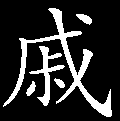
\includegraphics[width=3mm]{../Images/00005}不是同人,且莫浪作知心语。似假如真,事事应难许。着紧温存,白雪阳春曲。谁堪比?船上要离,未解奸侠起。}

话说王夫人听见邢夫人来了,连忙迎了出去。邢夫人犹不知贾母已知鸳鸯之事,正还要来打听信息,进了院门,早有几个婆子悄悄的回了他,他方知道。待要回去,里面已知,又见王夫人接了出来,少不得进来,先与贾母请安,贾母一声儿不言语,自己也觉得愧悔。凤姐儿早指一事回避了。鸳鸯也自回房去生气。薛姨妈王夫人等恐碍着邢夫人的脸面,也都渐渐的退了。邢夫人且不敢出去。

贾母见无人,方说道:``我听见你替你老爷说媒来了。你倒也三从四德,只是这贤慧也太过了!你们如今也是孙子儿子满眼了,你还怕他,劝两句都使不得,还由着你老爷性儿闹。''邢夫人满面通红,回道:``我劝过几次不依。老太太还有什么不知道呢,我也是不得已儿。''贾母道:``他逼着你杀人,你也杀去?如今你也想想,你兄弟媳妇本来老实,又生得多病多痛,上上下下那不是他操心?你一个媳妇虽然帮着,也是天天丢下笆儿弄扫帚。凡百事情,我如今都自己减了。他们两个就有一些不到的去处,有鸳鸯,那孩子还心细些,我的事情他还想着一点子,该要去的,他就要了来,该添什么,他就度空儿告诉他们添了。鸳鸯再不这样,他娘儿两个,里头外头,大的小的,那里不忽略一件半件,我如今反倒自己操心去不成?还是天天盘算和你们要东西去?我这屋里有的没的,剩了他一个,年纪也大些,我凡百的脾气性格儿他还知道些。二则他还投主子们的缘法,也并不指着我和这位太太要衣裳去,又和那位奶奶要银子去。所以这几年一应事情,他说什么,从你小婶和你媳妇起,以至家下大大小小,没有不信的。所以不单我得靠,连你小婶媳妇也都省心。我有了这么个人,便是媳妇和孙子媳妇有想不到的,我也不得缺了,也没气可生了。这会子他去了,你们弄个什么人来我使?你们就弄他那么一个真珠的人来,不会说话也无用。我正要打发人和你老爷说去,他要什么人,我这里有钱,叫他只管一万八千的买,就只这个丫头不能。留下他伏侍我几年,就比他日夜伏侍我尽了孝的一般。你来的也巧,你就去说,更妥当了。''

说毕,命人来:``请了姨太太、你姑娘们来说个话儿。才高兴,怎么又都散了!''丫头们忙答应着去了。众人忙赶的又来。只有薛姨妈向丫鬟道:``我才来了,又作什么去?你就说我睡了觉了。''那丫头道:``好亲亲的姨太太,姨祖宗!我们老太太生气呢,你老人家不去,没个开交了,只当疼我们罢。你老人家嫌乏,我背了你老人家去。''薛姨妈道:``小鬼头儿,你怕些什么?不过骂几句完了。''说着,只得和这小丫头子走来。贾母忙让坐,又笑道:``咱们斗牌罢。姨太太的牌也生,咱们一处坐着,别叫凤姐儿混了我们去。''薛姨妈笑道:``正是呢,老太太替我看着些儿。就是咱们娘儿四个斗呢,还是再添个呢?''王夫人笑道:``可不只四个。''{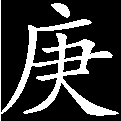
\includegraphics[width=3mm]{../Images/00004}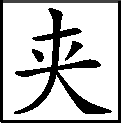
\includegraphics[width=3mm]{../Images/00012}\footnotesize \kaishu 老实人言语。}凤姐儿道:``再添一个人热闹些。''贾母道:``叫鸳鸯来,叫他在这下手里坐着。姨太太眼花了,咱们两个的牌都叫他瞧着些儿。''凤姐儿叹了一声,向探春道:``你们知书识字的,倒不学算命!''探春道:``这又奇了。这会子你倒不打点精神赢老太太几个钱,又想算命。''凤姐儿道:``我正要算算今儿该输多少呢,我还想赢呢!你瞧瞧,场子没上,左右都埋伏下了。''说的贾母薛姨妈都笑起来。

一时,鸳鸯来了,便坐在贾母下手,鸳鸯之下便是凤姐儿。铺下红毡,洗牌告幺,五人起牌。斗了一回,鸳鸯见贾母的牌已十严,只等一张二饼,便递了暗号与凤姐儿。凤姐儿正该发牌,便故意踌躇了半晌,笑道:``我这一张牌定在姨妈手里扣着呢。我若不发这一张,再顶不下来的。''薛姨妈道:``我手里并没有你的牌。''凤姐儿道:``我回来是要查的。''薛姨妈道:``你只管查。你且发下来,我瞧瞧是张什么。''凤姐儿便送在薛姨妈跟前。薛姨妈一看是个二饼,便笑道:``我倒不稀罕他,只怕老太太满了。''凤姐儿听了,忙笑道:``我发错了。''贾母笑的已掷下牌来,说:``你敢拿回去!谁叫你错的不成?''凤姐儿道:``可是我要算一算命呢。这是自己发的,也怨埋伏!''贾母笑道:``可是呢,你自己该打着你那嘴,问着你自己才是。''又向薛姨妈笑道:``我不是小器爱赢钱,原是个彩头儿。''薛姨妈笑道:``可不是这样,那里有那样糊涂人说老太太爱钱呢?''凤姐儿正数着钱,听了这话,忙又把钱穿上了,向众人笑道:``够了我的了。竟不为赢钱,单为赢彩头儿。我到底小器,输了就数钱,快收起来罢。''贾母规矩是鸳鸯代洗牌,因和薛姨妈说笑,不见鸳鸯动手,贾母道:``你怎么恼了,连牌也不替我洗。''鸳鸯拿起牌来,笑道:``二奶奶不给钱。''贾母道:``他不给钱,那是他交运了。''便命小丫头子:``把他那一吊钱都拿过来。''小丫头子真就拿了,搁在贾母旁边。凤姐儿笑道:``赏我罢,我照数儿给就是了。''薛姨妈笑道:``果然是凤丫头小器,不过是顽儿罢了。''凤姐听说,便站起来,拉着薛姨妈,回头指着贾母素日放钱的一个木匣子笑道:``姨妈瞧瞧,那个里头不知顽了我多少去了。这一吊钱顽不了半个时辰,那里头的钱就招手儿叫他了。只等把这一吊也叫进去了,牌也不用斗了,老祖宗的气也平了,又有正经事差我办去了。''话说未完,引的贾母众人笑个不住。偏有平儿怕钱不够,又送了一吊来。凤姐儿道:``不用放在我跟前,也放在老太太的那一处罢。一齐叫进去倒省事,不用做两次,叫箱子里的钱费事。''贾母笑的手里的牌撒了一桌子,推着鸳鸯,叫:``快撕他的嘴!''

平儿依言放下钱,也笑了一回,方回来。至院门前遇见贾琏,问他:``太太在那里呢?老爷叫我请过去呢。''平儿忙笑道:``在老太太跟前呢,站了这半日还没动呢。趁早儿丢开手罢。老太太生了半日气,这会子亏二奶奶凑了半日趣儿,才略好了些。''贾琏道:``我过去只说讨老太太的示下,十四往赖大家去不去,好预备轿子的。又请了太太,又凑了趣儿,岂不好?''平儿笑道:``依我说,你竟不去罢。合家子连太太宝玉都有了不是,这会子你又填限去了。''贾琏道:``已经完了,难道还找补不成?况且与我又无干。二则老爷亲自吩咐我请太太的,这会子我打发了人去,倘或知道了,正没好气呢,指着这个拿我出气罢。''说着就走。平儿见他说得有理,也便跟了过来。

贾琏到了堂屋里,便把脚步放轻了,往里间探头,只见邢夫人站在那里。凤姐儿眼尖,先瞧见了,使眼色儿不命他进来,又使眼色与邢夫人。邢夫人不便就走,只得倒了一碗茶来,放在贾母跟前。贾母一回身,贾琏不防,便没躲伶俐。贾母便问:``外头是谁?倒像个小子一伸头。''凤姐儿忙起身说:``我也恍惚看见一个人影儿,让我瞧瞧去。''一面说,一面起身出来。贾琏忙进去,陪笑道:``打听老太太十四可出门?好预备轿子。''贾母道:``既这么样,怎么不进来?又作鬼作神的。''贾琏陪笑道:``见老太太玩牌,不敢惊动,不过叫媳妇出来问问。''贾母道:``就忙到这一时,等他家去,你问多少问不得?那一遭儿你这么小心来着!又不知是来作耳报神的,也不知是来作探子的,鬼鬼祟祟的,倒唬了我一跳。什么好下流种子!你媳妇和我顽牌呢,还有半日的空儿,你家去再和那赵二家的商量治你媳妇去罢!''说着,众人都笑了。鸳鸯笑道:``鲍二家的,老祖宗又拉上赵二家的。''贾母也笑道:``可是,我那里记得什么抱着背着的,提起这些事来,不由我不生气!我进了这门子作重孙子媳妇起,到如今我也有了重孙子媳妇了,连头带尾五十四年,凭着大惊大险千奇百怪的事,也经了些,从没经过这些事。还不离了我这里呢!''

贾琏一声儿不敢说,忙退了出来。平儿站在窗外悄悄的笑道:``我说着你不听,到底碰在网里了。''正说着,只见邢夫人也出来,贾琏道:``都是老爷闹的,如今都搬在我和太太身上。''邢夫人道:``我把你没孝心雷打的下流种子!人家还替老子死呢,白说了几句,你就抱怨了。你还不好好的呢,这几日生气,仔细他捶你。''贾琏道:``太太快过去罢,叫我来请了好半日了。''说着,送他母亲出来过那边去。

邢夫人将方才的话只略说了几句,贾赦无法,又含愧,自此便告病,且不敢见贾母,只打发邢夫人及贾琏每日过去请安。只得又各处遣人购求寻觅,终究费了八百两银子买了一个十七岁的女孩子来,名唤嫣红,收在屋内。不在话下。

这里斗了半日牌,吃晚饭才罢。此一二日间无话。

展眼到了十四日,黑早,赖大的媳妇又进来请。贾母高兴,便带了王夫人薛姨妈及宝玉姊妹等,到赖大花园中坐了半日。那花园虽不及大观园,却也十分齐整宽阔,泉石林木,楼阁亭轩,也有好几处惊人骇目的。外面厅上,薛蟠、贾珍、贾琏、贾蓉并几个近族的,很远的也没来,贾赦也没来。赖大家内也请了几个现任的官长并几个世家子弟作陪。因其中有柳湘莲,薛蟠自上次会过一次,已念念不忘。又打听他最喜串戏,且串的都是生旦风月戏文,不免错会了意,误认他作了风月子弟,正要与他相交,恨没有个引进,这日可巧遇见,竟觉无可不可。且贾珍等也慕他的名,酒盖住了脸,就求他串了两出戏。下来,移席和他一处坐着,问长问短,说此说彼。

那柳湘莲原是世家子弟,读书不成,父母早丧,素性爽侠,不拘细事,酷好耍枪舞剑,赌博吃酒,以至眠花卧柳,吹笛弹筝,无所不为。因他年纪又轻,生得又美,不知他身分的人,却误认作优伶一类。那赖大之子赖尚荣与他素习交好,故他今日请来作陪。不想酒后别人犹可,独薛蟠又犯了旧病。他心中早已不快,得便意欲走开完事,无奈赖尚荣死也不放。赖尚荣又说:``方才宝二爷又嘱咐我,才一进门虽见了,只是人多不好说话,叫我嘱咐你散的时候别走,他还有话说呢。你既一定要去,等我叫出他来,你两个见了再走,与我无干。''说着,便命小厮们到里头找一个老婆子,悄悄告诉``请出宝二爷来。''那小厮去了没一盏茶时,果见宝玉出来了。赖尚荣向宝玉笑道:``好叔叔,把他交给你,我张罗人去了。''说着,一径去了。

宝玉便拉了柳湘莲到厅侧小书房中坐下,问他这几日可到秦钟的坟上去了。{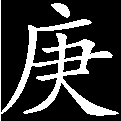
\includegraphics[width=3mm]{../Images/00004}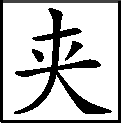
\includegraphics[width=3mm]{../Images/00012}\footnotesize \kaishu 忽提此人,使我堕泪。近几回不见提此人,自谓不表矣。乃忽于此处柳湘莲提及,所谓``方以类聚,物以群分''也。}湘莲道:``怎么不去?前日我们几个人放鹰去,离他坟上还有二里,我想今年夏天的雨水勤,恐怕他的坟站不住。我背着众人,走去瞧了一瞧,果然又动了一点子。回家来就便弄了几百钱,第三日一早出去,雇了两个人收拾好了。''宝玉道:``怪道呢,上月我们大观园的池子里头结了莲蓬,我摘了十个,叫茗烟出去到坟上供他去,回来我也问他可被雨冲坏了没有。他说不但不冲,且比上回又新了些。我想着,不过是这几个朋友新筑了。我只恨我天天圈在家里,一点儿做不得主,行动就有人知道,不是这个拦就是那个劝的,能说不能行。虽然有钱,又不由我使。''湘莲道:``这个事也用不着你操心,外头有我,你只心里有了就是。眼前十月一,我已经打点下上坟的花消。你知道我一贫如洗,家里是没的积聚,纵有几个钱来,随手就光的,不如趁空儿留下这一分,省得到了跟前扎煞手。''宝玉道:``我也正为这个要打发茗烟找你,你又不大在家,知道你天天萍踪浪迹,没个一定的去处。''湘莲道:``这也不用找我。这个事不过各尽其道。眼前我还要出门去走走,外头逛个三年五载再回来。''宝玉听了,忙问道:``这是为何?''柳湘莲冷笑道:``你不知道我的心事,等到跟前你自然知道。我如今要别过了。''宝玉道:``好容易会着,晚上同散岂不好?''湘莲道:``你那令姨表兄还是那样,再坐着未免有事,不如我回避了倒好。''宝玉想了一想,道:``既是这样,倒是回避他为是。只是你要果真远行,必须先告诉我一声,千万别悄悄的去了。''说着便滴下泪来。柳湘莲道:``自然要辞的。你只别和别人说就是。''说着便站起来要走,又道:``你们进去,不必送我。''一面说,一面出了书房。

刚至大门前,早遇见薛蟠在那里乱嚷乱叫说:``谁放了小柳儿走了!''柳湘莲听了,火星乱迸,恨不得一拳打死,复思酒后挥拳,又碍着赖尚荣的脸面,只得忍了又忍。薛蟠忽见他走出来,如得了珍宝,忙趔趄着上来一把拉住,笑道:``我的兄弟,你往那里去了?''湘莲道:``走走就来。''薛蟠笑道:``好兄弟,你一去都没兴了,好歹坐一坐,你就疼我了。凭你有什么要紧的事,交给哥,你只别忙,有你这个哥,你要做官发财都容易。''湘莲见他如此不堪,心中又恨又愧,早生一计,便拉他到避人之处,笑道:``你真心和我好,假心和我好呢?''薛蟠听这话,喜的心痒难挠,乜斜着眼忙笑道:``好兄弟,你怎么问起我这话来?我要是假心,立刻死在眼前!''湘莲道:``既如此,这里不便。等坐一坐,我先走,你随后出来,跟到我下处,咱们替另喝一夜酒。我那里还有两个绝好的孩子,从没出门。你可连一个跟的人也不用带,到了那里,伏侍的人都是现成的。''薛蟠听如此说,喜得酒醒了一半,说:``果然如此?''湘莲道:``如何!人拿真心待你,你倒不信了!''薛蟠忙笑道:``我又不是呆子,怎么有个不信的呢!既如此,我又不认得,你先去了,我在那里找你?''湘莲道:``我这下处在北门外头,你可舍得家,城外住一夜去?''薛蟠笑道:``有了你,我还要家做什么!''湘莲道:``既如此,我在北门外头桥上等你。咱们席上且吃酒去。你看我走了之后你再走,他们就不留心了。''薛蟠听了,连忙答应。于是二人复又入席,饮了一回。那薛蟠难熬,只拿眼看湘莲,心内越想越乐,左一壶右一壶,并不用人让,自己便吃了又吃,不觉酒已八九分了。

湘莲便起身出来,瞅人不防去了,至门外,命小厮杏奴:``先家去罢,我到城外就来。''说毕,已跨马直出北门,桥上等候薛蟠。没顿饭时工夫,只见薛蟠骑着一匹大马,远远的赶了来,张着嘴,瞪着眼,头似拨浪鼓一般不住左右乱瞧。及至从湘莲马前过去,只顾望远处瞧,不曾留心近处,反踩过去了。湘莲又是笑,又是恨,便也撒马随后赶来。薛蟠往前看时,渐渐人烟稀少,便又圈马回来再找,不想一回头见了湘莲,如获奇珍,忙笑道:``我说你是个再不失信的。''湘莲笑道:``快往前走,仔细人看见跟了来,就不便了。''说着,先就撒马前去,薛蟠也紧紧跟来。

湘莲见前面人迹已稀,且有一带苇塘,便下马,将马拴在树上,向薛蟠笑道:``你下来,咱们先设个誓,日后要变了心,告诉人去的,便应了誓。''薛蟠笑道:``这话有理。''连忙下了马,也拴在树上,便跪下说道:``我要日久变心,告诉人去的,天诛地灭!''一语未了,只听``嘡''的一声,颈后好似铁锤砸下来,只觉得一阵黑,满眼金星乱迸,身不由己,便倒下来。湘莲走上来瞧瞧,知道他是个笨家,不惯捱打,只使了三分气力,向他脸上拍了几下,登时便开了果子铺。薛蟠先还要挣挫起来,又被湘莲用脚尖点了两点,仍旧跌倒,口内说道:``原是两家情愿,你不依,只好说,为什么哄出我来打我?''一面说,一面乱骂。湘莲道:``我把你瞎了眼的,你认认柳大爷是谁!你不说哀求,你还伤我!我打死你也无益,只给你个利害罢。''说着,便取了马鞭过来,从背至胫,打了三四十下。薛蟠酒已醒了大半,觉得疼痛难禁,不禁有``嗳哟''之声。湘莲冷笑道:``也只如此!我只当你是不怕打的。''一面说,一面又把薛蟠的左腿拉起来,朝苇中泞泥处拉了几步,滚的满身泥水,又问道:``你可认得我了?''薛蟠不应,只伏着哼哼。湘莲又掷下鞭子,用拳头向他身上擂了几下。薛蟠便乱滚乱叫,说:``肋条折了。我知道你是正经人,因为我错听了旁人的话了。''湘莲道:``不用拉别人,你只说现在的。''薛蟠道:``现在没什么说的。不过你是个正经人,我错了。''湘莲道:``还要说软些才饶你。''薛蟠哼哼着道:``好兄弟。''湘莲便又一拳。薛蟠``嗳哟''了一声道:``好哥哥。''湘莲又连两拳。薛蟠忙``嗳哟''叫道:``好老爷,饶了我这没眼睛的瞎子罢!从今以后我敬你怕你了。''湘涟道:``你把那水喝两口!''薛蟠一面听了,一面皱眉道:``那水脏得很,怎么喝得下去!''湘莲举拳就打。薛蟠忙道:``我喝,喝。''说着,只得俯头向苇根下喝了一口,犹未咽下去,只听``哇''的一声,把方才吃的东西都吐了出来。湘莲道:``好脏东西,你快吃尽了饶你。''薛蟠听了,叩头不迭道:``好歹积阴功饶我罢!这至死不能吃的。''湘莲道:``这样气息,倒薰坏了我。''说着丢了薛蟠,便牵马认镫去了。这里薛蟠见他已去,方放下心来,后悔自己不该误认了人。待要挣挫起来,无奈遍身疼痛难禁。

谁知贾珍等席上忽然不见了他两个,各处寻找不见。有人说:``恍惚出北门去了。''薛蟠的小厮们素日是惧他的,他吩咐不许跟去,谁还敢找去?{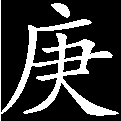
\includegraphics[width=3mm]{../Images/00004}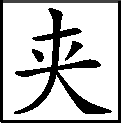
\includegraphics[width=3mm]{../Images/00012}\footnotesize \kaishu 亦如秦法自误。}后来还是贾珍不放心,命贾蓉带着小厮们寻踪问迹的直找出北门,下桥二里多路,忽见苇坑边薛蟠的马拴在那里。众人都道:``可好了!有马必有人。''一齐来至马前,只听苇中有人呻吟。大家忙走来一看,只见薛蟠衣衫零碎,面目肿破,没头没脸,遍身内外,滚的似个泥猪一般。贾蓉心内已猜着九分了,忙下马令人搀了出来,笑道:``薛大叔天天调情,今儿调到苇子坑里来了。必定是龙王爷也爱上你风流,要你招驸马去,你就碰到龙犄角上了。''薛蟠羞的恨没地缝儿钻不进去,那里爬的上马去?贾蓉只得命人赶到关厢里雇了一乘小轿子,薛蟠坐了,一齐进城。贾蓉还要抬往赖家去赴席,薛蟠百般央告,又命他不要告诉人,贾蓉方依允了,让他各自回家。贾蓉仍往赖家回复贾珍,并说方才形景。贾珍也知为湘莲所打,也笑道:``他须得吃个亏才好。''至晚散了,便来问候。薛蟠自在卧房将养,推病不见。

贾母等回来各自归家时,薛姨妈与宝钗见香菱哭得眼睛肿了。问其原故,忙赶来瞧薛蟠时,脸上身上虽有伤痕,并未伤筋动骨。薛姨妈又是心疼,又是发恨,骂一回薛蟠,又骂一回柳湘莲,意欲告诉王夫人,遣人寻拿柳湘莲。宝钗忙劝道:``这不是什么大事,不过他们一处吃酒,酒后反脸常情。谁醉了,多挨几下子打,也是有的。况且咱们家无法无天,也是人所共知的。妈不过是心疼的缘故。要出气也容易,等三五天哥哥养好了出的去时,那边珍大爷琏二爷这干人也未必白丢开了,自然备个东道,叫了那个人来,当着众人替哥哥赔不是认罪就是了。如今妈先当件大事告诉众人,倒显得妈偏心溺爱,纵容他生事招人,今儿偶然吃了一次亏,妈就这样兴师动众,倚着亲戚之势欺压常人。''薛姨妈听了道:``我的儿,到底是你想的到,我一时气糊涂了。''宝钗笑道:``这才好呢。他又不怕妈,又不听人劝,一天纵似一天,吃过两三个亏,他倒罢了。''

薛蟠睡在炕上,痛骂柳湘莲,又命小厮们去拆他的房子,打死他,和他打官司。薛姨妈禁住小厮们,只说柳湘莲一时酒后放肆,如今酒醒,后悔不及,惧罪逃走了。薛蟠听见如此说了,要知端的------

{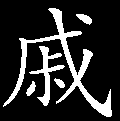
\includegraphics[width=3mm]{../Images/00005}总评:自斗牌一节,写贵家长上之尊重,卑幼之侍奉;遭打一节,写薛蟠之呆,湘莲之豪,薛母、宝钗之言,无不逼真。}
